\section{Results}
\label{sec:results}
LETT-NeXt was evaluated in terms of segmentation accuracy, qualitative behavior, and computational efficiency. 
Quantitative performance was measured on the public validation set and hidden test set using DSC, NSD, and the challenge score. Metrics are reported on a 0--100 scale, and absolute differences are reported in percentage points.


\subsection{Quantitative validation results}

LETT-NeXt completed all 49 public validation cases without failures or timeouts. 
Table~\ref{tab:final-results} summarizes public validation and hidden test performance. 
Compared with the Lite ENSAM competition baseline, LETT-NeXt achieved higher hidden test DSC, NSD, and challenge score. 
LETT-NeXt also achieved higher public-validation DSC, NSD, and score. Lite ENSAM validation values follow the corrected local evaluation reported in its repository\footnote{\url{https://github.com/Ahus-AIM/FLARE25}}.

\begin{table}[htbp]
\caption{Quantitative evaluation results on the public validation and hidden test sets. The LETT-NeXt validation result uses the inference pipeline with AutoZoom enabled. Lite ENSAM's validation score is approximated from its rounded DSC and NSD means.}
\label{tab:final-results}
\centering
\begin{adjustbox}{max width=\linewidth}
\begin{tabular}{lcccccc}
\toprule
\multirow{2}{*}{Model} & \multicolumn{3}{c}{Public Validation} & \multicolumn{3}{c}{Hidden Test} \\
\cmidrule(lr){2-4} \cmidrule(lr){5-7}
                         & DSC(\%) & NSD(\%) & Score(\%) & DSC(\%) & NSD(\%) & Score(\%) \\
\midrule
Lite ENSAM               & $69.7 \pm 16.8$ & $61.8 \pm 19.1$ & $\approx 65.8$            & $60.70$ & $63.60$ & $62.15$ \\
LETT-NeXt                & $79.43 \pm 10.09$ & $72.32 \pm 16.22$ & $75.87 \pm 12.17$ & $73.90$ & $67.30$ & $70.60$ \\
\bottomrule
\end{tabular}
\end{adjustbox}
\end{table}

The larger standard deviation for NSD suggests that boundary accuracy varied more than volumetric overlap.
However, the numerical ordering of DSC and NSD alone does not establish under-segmentation.


\subsection{Qualitative results}

\Cref{fig:percentile_examples} shows representative validation examples selected by score percentile. Qualitatively, LETT-NeXt usually localized the prompted lesion, but the main visible failure mode was under-segmentation. In difficult cases, the model predicted masks that were too small, especially for small lesions, low-contrast lesions, and lesions with unclear boundaries.

\begin{figure}[htbp]
    \centering
    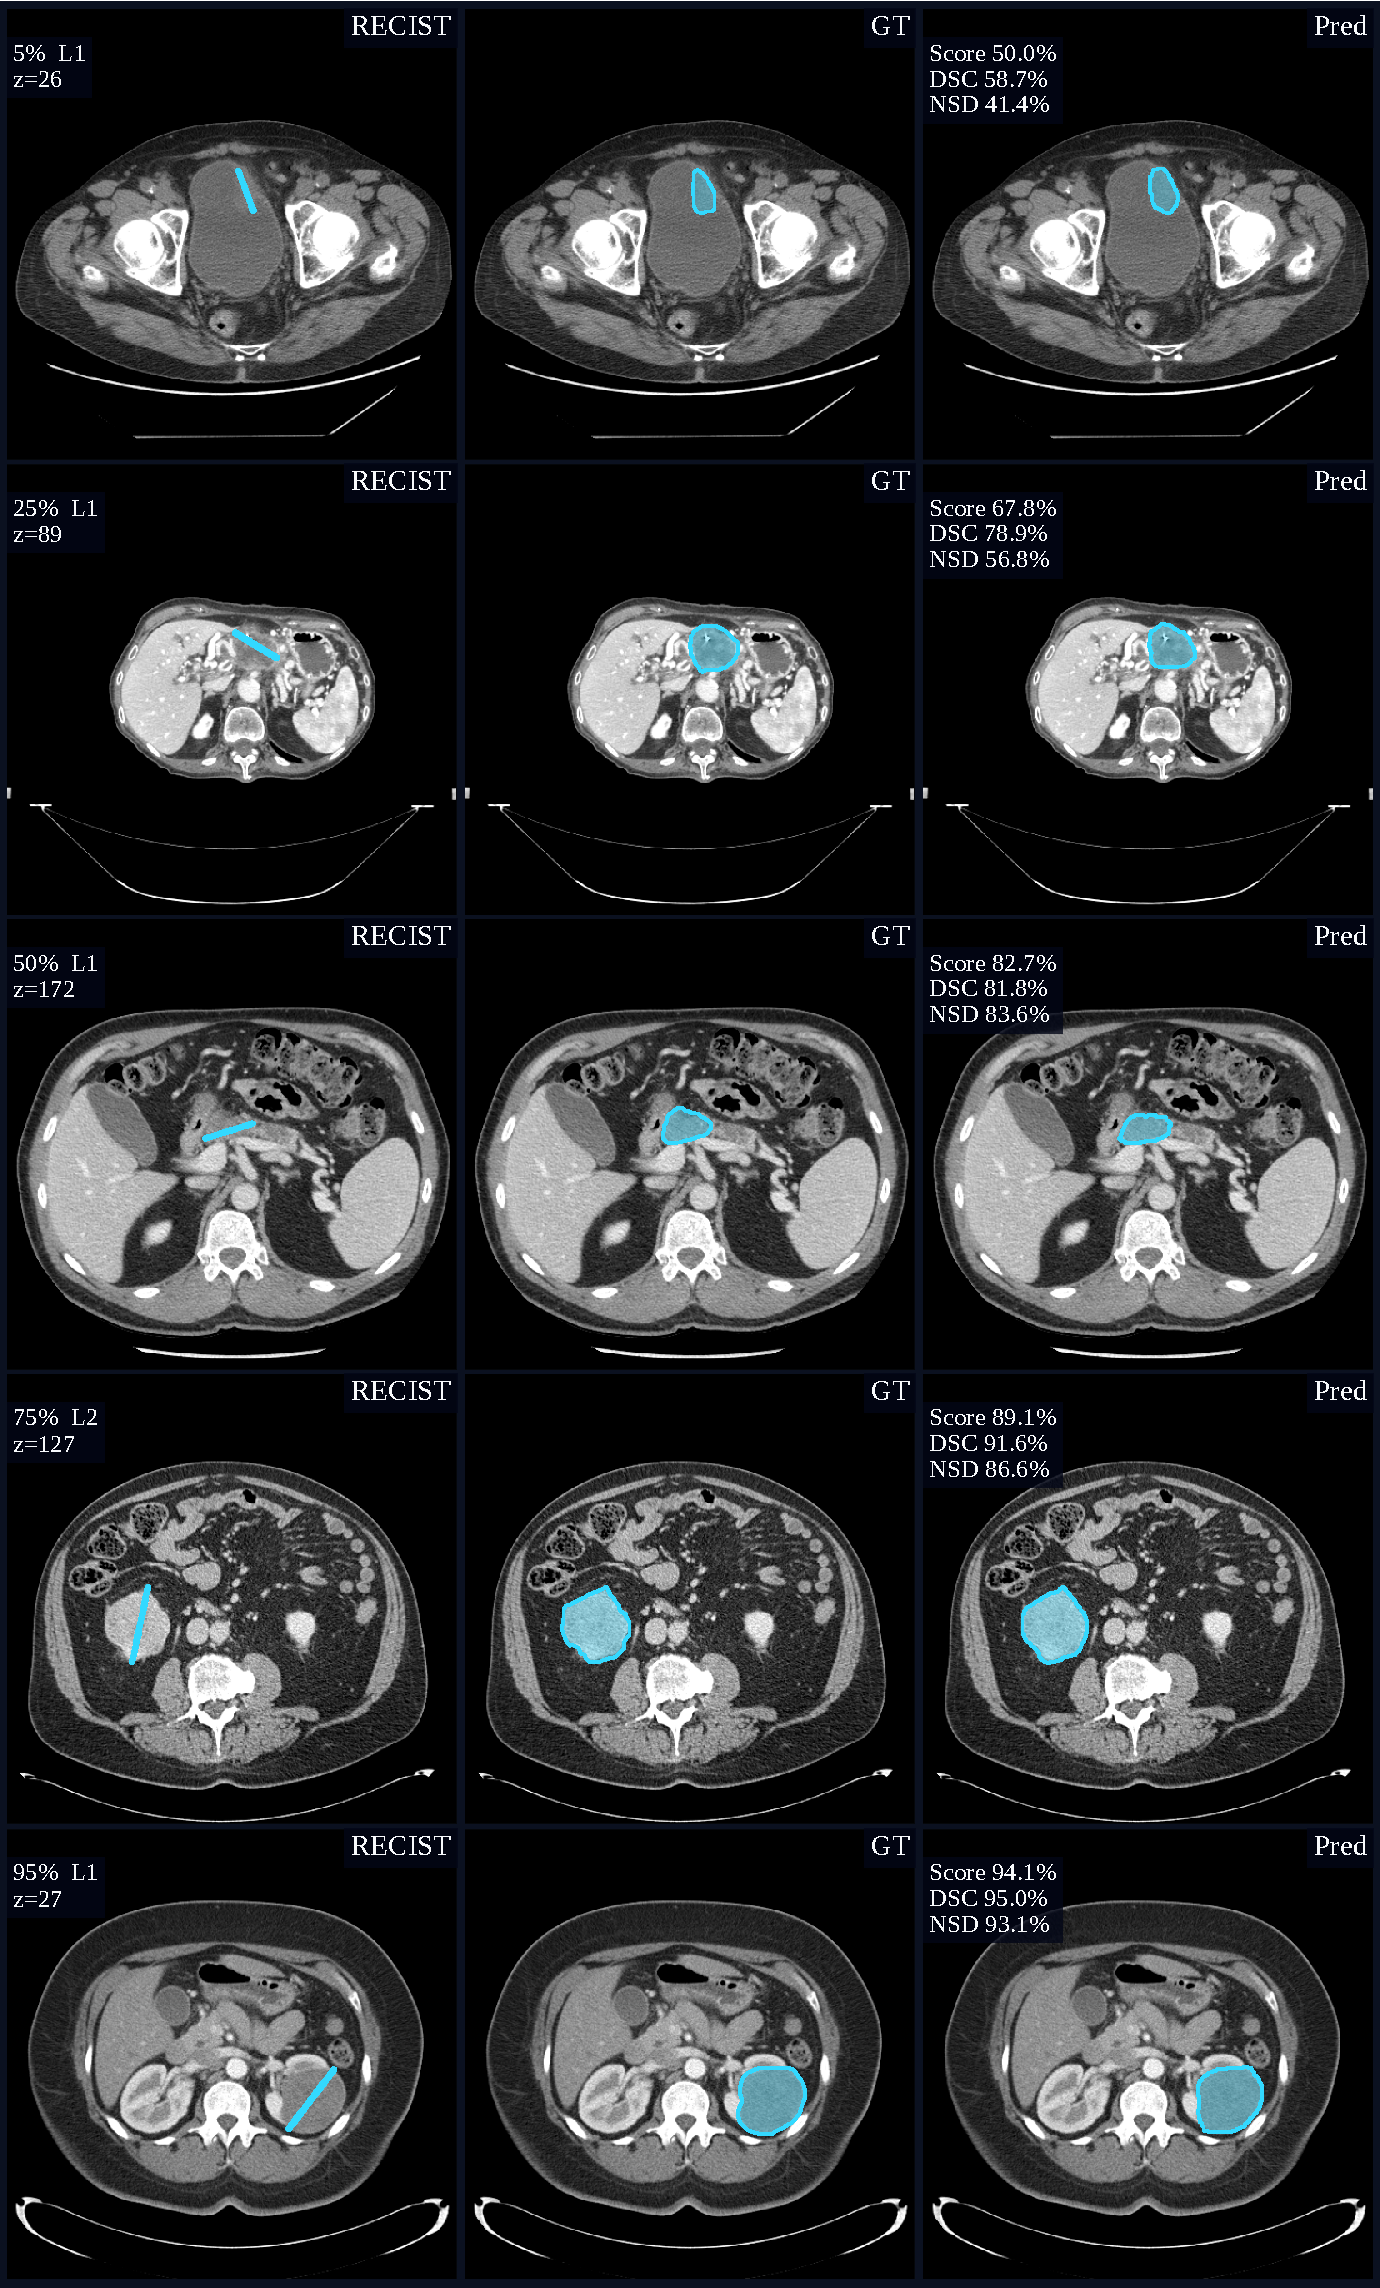
\includegraphics[width=\linewidth,height=0.72\textheight,keepaspectratio]{images/percentile_segmentation_examples_full_v2.pdf}
    \caption{
    Qualitative validation examples across score percentiles. 
    Each row shows the RECIST input marker, ground-truth mask, and LETT-NeXt prediction on the prompt slice. 
    Higher-score examples generally show stronger agreement with the ground truth. 
    }
    \label{fig:percentile_examples}
\end{figure}

\subsection{Runtime and memory}

LETT-NeXt satisfied the CPU inference constraints on the 49-case public validation set. 
Table~\ref{tab:efficiency_results} summarizes validation set runtime and memory use. 
The hidden test server reported a mean runtime of \(20.9\,\mathrm{s}\) per case under hidden challenge-server conditions.

\begin{table}[htbp]
    \centering
    \caption{Runtime and memory use on the 49-case public validation set.}
    \label{tab:efficiency_results}
    \begin{adjustbox}{max width=\linewidth}
\begin{tabular}{ll}
        \toprule
        \textbf{Quantity} & \textbf{Value} \\
        \midrule
        Mean runtime per case & \(6.88 \pm 3.00\,\mathrm{s}\) \\
        Maximum runtime & \(13.55\,\mathrm{s}\) \\
        Mean CPU memory-time & \(11.01 \pm 5.49\,\mathrm{GB\,s}\) \\
        Total CPU memory-time & \(539.36\,\mathrm{GB\,s}\) \\
        Maximum resident memory & \(3.57\,\mathrm{GB}\) \\
        \bottomrule
    \end{tabular}
\end{adjustbox}
\end{table}

